\section{Desarrollo } 

MODELOS DIMENSIONAL
\begin{itemize}

\item Tarea 1 :
El siguiente diagrama E / R simplificado describe el envío de mercancías. Los lotes pertenecientes a ciertos grupos se
envían a ciertos destinos en varios países a través de diferentes modos de transporte. Un cierto centro de costos es
responsable de cada envío

\begin{center}
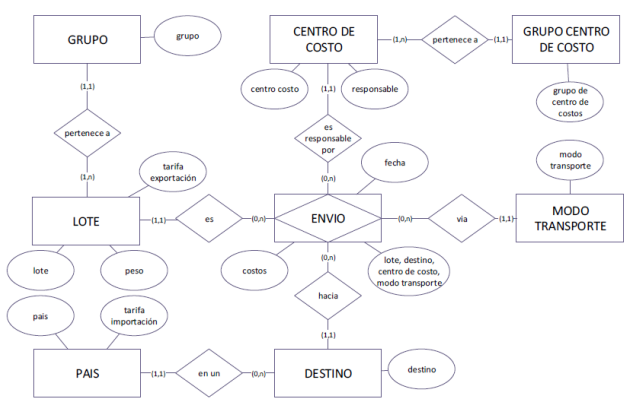
\includegraphics[width=14cm]{./Imagenes/tarea1.png}
\end{center}

Realizacion de Modelo fìsico de diagrama entidad - relacion

\begin{center}
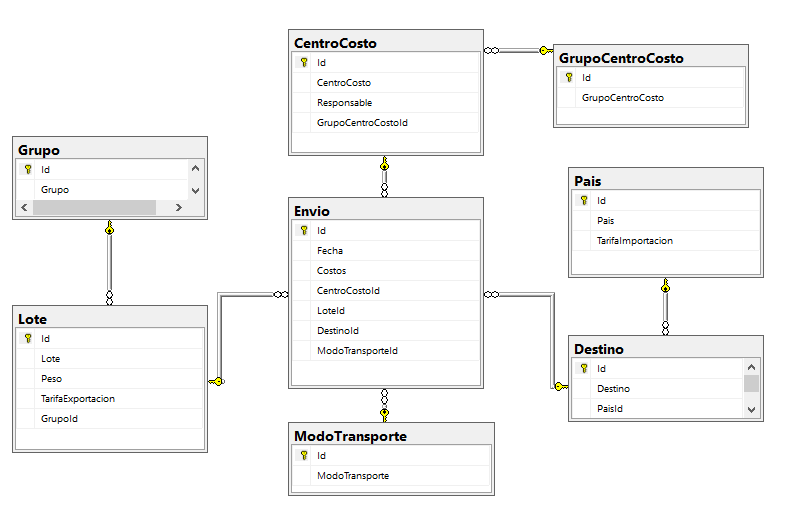
\includegraphics[width=14cm]{./Imagenes/tarea111.png}
\end{center}

Realizacion del  Modelo Dimensional 

\begin{center}
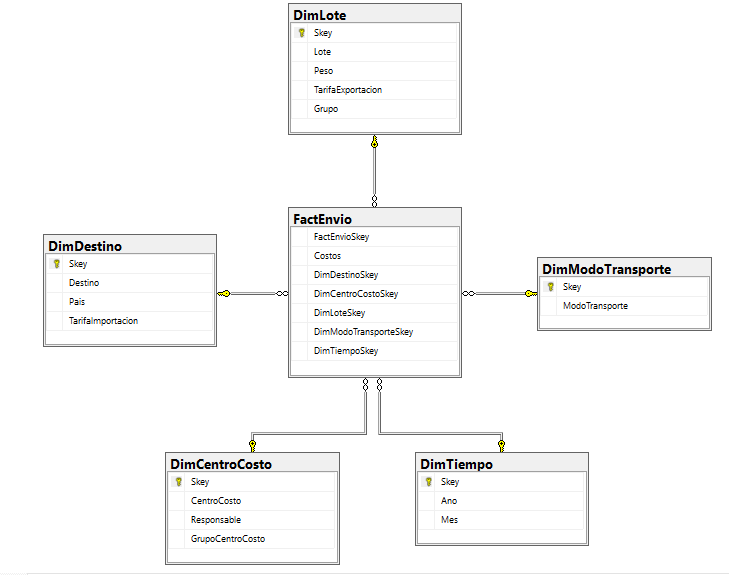
\includegraphics[width=14cm]{./Imagenes/tarea11.png}
\end{center}


\item Tarea 2 :
En este esquema de E / R, un cliente (que es de cierto tipo) reserva un viaje en una agencia de viajes. La agencia de viajes
trabaja para un determinado operador turístico. El viaje va a un destino determinado que pertenece a un país determinado.

\begin{center}
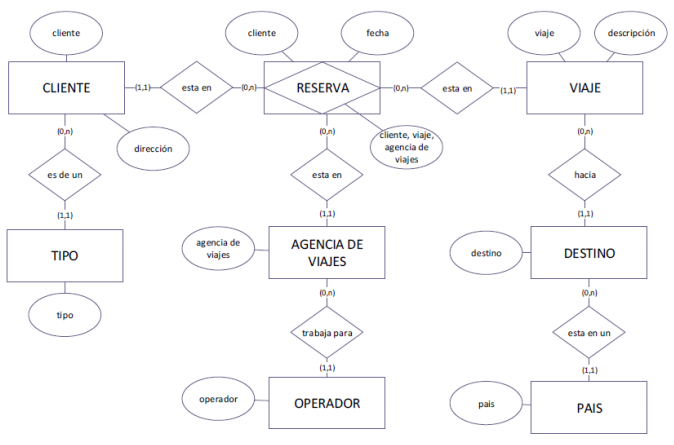
\includegraphics[width=14cm]{./Imagenes/tarea2.png}
\end{center}

Realizacion del Modelo fìsico de diagrama entidad - relacion

\begin{center}
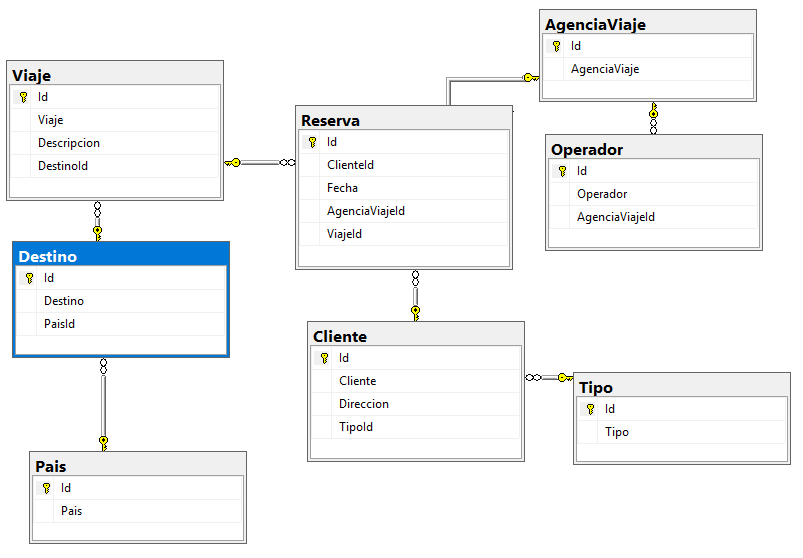
\includegraphics[width=14cm]{./Imagenes/tarea222.png}
\end{center}


 Realizacion del Modelo Dimensional 

\begin{center}
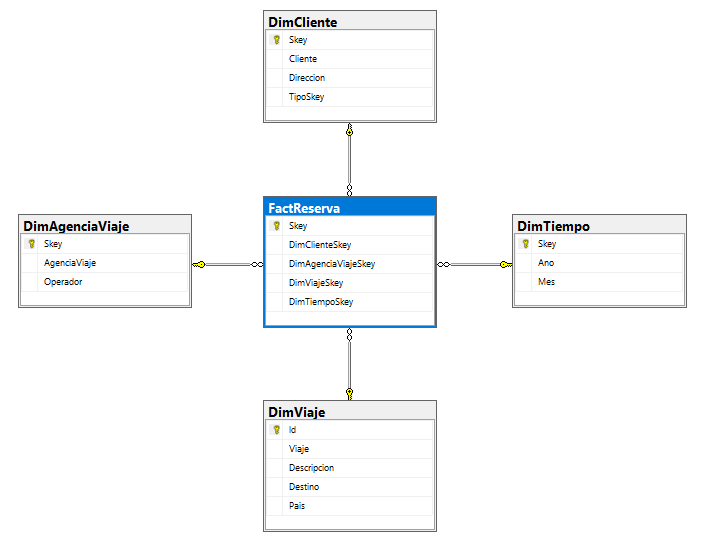
\includegraphics[width=14cm]{./Imagenes/tarea22.png}
\end{center}


\item Tarea 3 :
Este esquema E / R simplificado muestra un caso gestión del proyecto.
El proyecto para un cliente se divide en varios paquetes de trabajo y siempre una persona es responsable de completar la
tarea. Se cuida en un lugar determinado.

\begin{center}
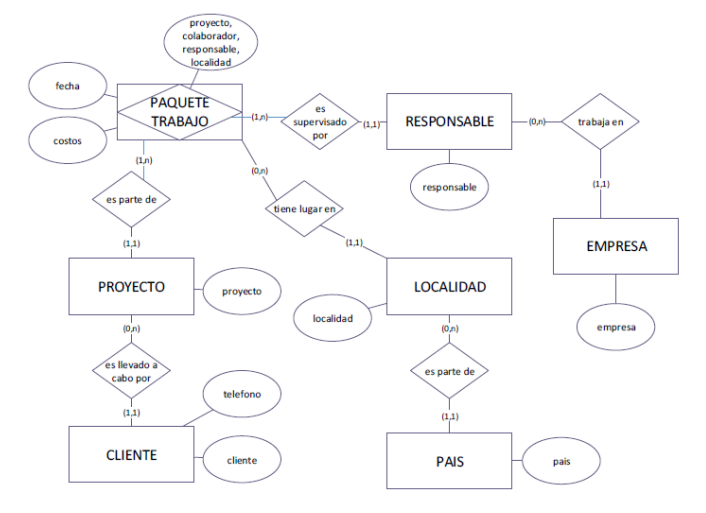
\includegraphics[width=16cm]{./Imagenes/tarea3.png}
\end{center}

Realizacion del Modelo fìsico de diagrama entidad - relacion

\begin{center}
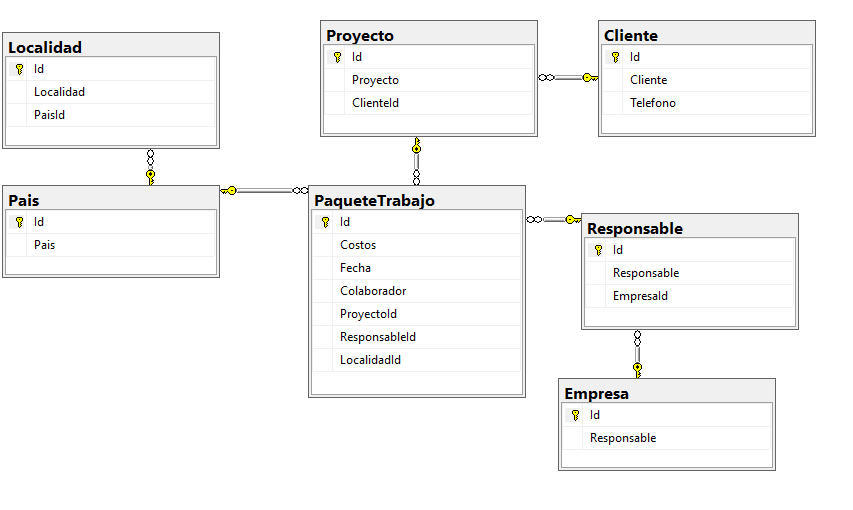
\includegraphics[width=15cm]{./Imagenes/tarea333.png}
\end{center}

 Realizacion del Modelo Dimensional 
\begin{center}
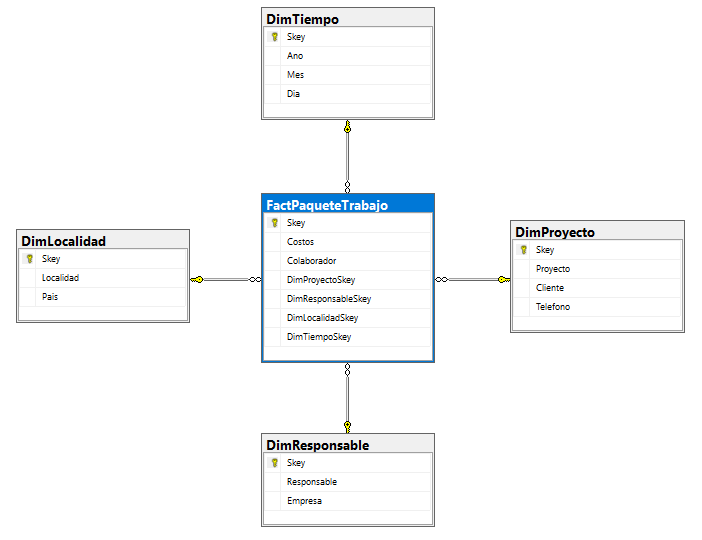
\includegraphics[width=14cm]{./Imagenes/tarea33.png}
\end{center}


\end{itemize}







